\documentclass[11pt,a4paper]{article}
\usepackage[utf8]{inputenc}
\usepackage[margin=1in]{geometry}
\usepackage{amsmath,amssymb,amsthm}
\usepackage{booktabs}
\usepackage{graphicx}
\usepackage{xcolor}
\usepackage{tikz}
\usetikzlibrary{shapes.geometric, arrows.meta, positioning, calc, fit, backgrounds}
\usepackage{microtype}
\usepackage{hyperref}
\usepackage{natbib}
\usepackage{subcaption}
\usepackage{enumitem}

\hypersetup{
    colorlinks=true,
    linkcolor=blue,
    citecolor=blue,
    urlcolor=blue
}

\newtheorem{definition}{Definition}
\newtheorem{axiom}{Axiom}
\newtheorem{proposition}{Proposition}

\title{\textbf{Ny\=aya-Pram\=a\d{n}a: A Neuro-Symbolic Epistemic Verification Framework for Calibrated, Provenance-Aware LLM Reasoning}}

\author{
  \textbf{Nitish Rajguru} \\
  Independent Researcher \\
  \texttt{nitishr655@gmail.com}
}

\date{\today}

\begin{document}

\maketitle

\begin{abstract}
Large Language Models (LLMs) demonstrate exceptional generative fluency but suffer from critical epistemic vulnerabilities: severe overconfidence on ungrounded propositions, inability to differentiate direct empirical observation from unverified textual hearsay (modality flattening), susceptibility to sycophantic hallucinations, and lack of mechanisms to invalidate obsolete beliefs. While retrieval-augmented generation and tool-use frameworks mitigate some factual errors, they lack a principled epistemic hierarchy to constrain subjective beliefs or invalidate flawed deductive steps.

In this paper, we introduce \textbf{Ny\=aya-Pram\=a\d{n}a}, a neuro-symbolic epistemic verification framework rooted in classical Ny\=aya-Vai\'se\d{s}ika epistemology. Ny\=aya-Pram\=a\d{n}a enforces a dual-system cognitive architecture: an unconstrained System~1 LLM proposer (\textit{Manas}) generates structured 5-part deductive arguments (\textit{Pa\~nc\=avayava}), which are audited by a deterministic System~2 epistemic verifier (\textit{Buddhi}). The verifier enforces a six-tier evidence modality hierarchy (\textit{Pram\=a\d{n}a}), applies empirical confidence ceilings, intercepts seven cognitive fallacies (\textit{Adhy\=asa}), validates causal claims via interventional $do$-calculus simulations, and updates a semantic vector belief store (\textit{Citta}) equipped with automated truth sublation (\textit{B\=adha}).

Across empirical evaluations, our framework demonstrates:
(1)~\textbf{Calibrated Confidence}: Achieves an Expected Calibration Error (ECE) of \textbf{0.0670} and a Brier Score of \textbf{0.1727}, outperforming standard uncalibrated LLM overconfidence ($\text{ECE} > 0.25$);
(2)~\textbf{Fallacy Interception}: Intercepts \textbf{100.0\%} of adversarial queries across 50 benchmark cases spanning correlation-causation confusion, scope inflation, sycophancy, and hearsay misattribution;
(3)~\textbf{Calibrated Abstention on TruthfulQA}: Correctly abstains on \textbf{40.0\%} of ungrounded or subjective queries with machine-readable codes, while verifying ground-truth scientific claims with zero conversational hallucination.
\end{abstract}

\section{Introduction}

Generative Large Language Models (LLMs) operate as statistical pattern matchers over autoregressive token distributions. While scaling model parameters and reinforcement learning from human feedback (RLHF) improve conversational coherence, they fail to resolve four fundamental epistemic defects:
\begin{enumerate}[leftmargin=*]
    \item \textbf{Modality Flattening}: Models treat direct empirical evidence (e.g., Python execution outputs, sensor measurements) and conversational hearsay with identical epistemic weight.
    \item \textbf{Unbounded Overconfidence}: Autoregressive models routinely state falsehoods with subjective confidence exceeding 90\%, yielding high Expected Calibration Error \citep{guo2017calibration}.
    \item \textbf{Cognitive Fallacies \& Sycophancy (\textit{Adhy\=asa})}: Models frequently echo user biases (asker projection) and conflate correlation with causation \citep{perez2022discovering,sharma2023sycophancy}.
    \item \textbf{Monotonic Epistemic Accumulation}: Vector databases accumulate beliefs monotonically without formal mechanisms to invalidate outdated or disproven facts.
\end{enumerate}

To address these vulnerabilities, we draw upon the formal epistemological school of classical Indian logic: the \textbf{Ny\=aya-Vai\'se\d{s}ika} tradition \citep{matilal1986perception,mohanty2000classical}. Developed over two millennia ago, Ny\=aya established that a cognition constitutes valid knowledge (\textit{pram\=a}) only when generated by an accredited cognitive instrument (\textit{pram\=a\d{n}a}). Furthermore, Ny\=aya formalizes a 5-part deductive argument (\textit{pa\~nc\=avayava}), a taxonomy of fallacies (\textit{adhy\=asa}), and the principle of sublation (\textit{b\=adha})---whereby an earlier cognition is cancelled upon encountering superior defeating evidence.

\section{Formal Epistemic Framework}

\begin{definition}[Structured Epistemic Claim]
A claim proposition is formally defined as an 8-tuple:
\begin{equation}
\mathcal{C} = \langle p, h, u, a, n, \pi, \kappa_0, \alpha \rangle
\end{equation}
where $p$ is the thesis (\textit{Pratij\~n\=a}), $h$ is the ground reason (\textit{Hetu}), $u$ is the universal invariant rule (\textit{Ud\=ahara\d{n}a}), $a$ is the application (\textit{Upanaya}), $n$ is the conclusion (\textit{Nigamana}), $\pi \in \Pi$ is the verification modality (\textit{Pram\=a\d{n}a}), $\kappa_0 \in [0, 1]$ is the proposer confidence, and $\alpha \in \{0, 1\}$ is the abstention flag.
\end{definition}

\begin{definition}[Pram\=a\d{n}a Modality Hierarchy and Ceilings]
Let $\Pi$ be the ordered set of evidence modalities, each bounded by an empirical ceiling $\kappa_{\max}(\pi)$:
\begin{equation}
\Pi = \{ \text{pratyak\d{s}a}~(0.95),~\text{anum\=ana}~(0.85),~\text{sabda}~(0.80),~\text{anupalabdhi}~(0.70),~\text{arth\=apatti}~(0.65),~\text{upam\=ana}~(0.60) \}
\end{equation}
\end{definition}

\begin{axiom}[Monotonic Confidence Bounding]
For any claim $\mathcal{C}$ asserting modality $\pi$, the calibrated confidence $\kappa'$ is strictly bounded by:
\begin{equation}
\kappa' \le \kappa_{\max}(\pi)
\end{equation}
\end{axiom}

\begin{definition}[Epistemic Calibration Operator]
Given detected fallacies $\mathcal{A} \subseteq \{a_1, \dots, a_7\}$, the calibrated confidence $\kappa_{\text{calibrated}}$ is computed by:
\begin{equation}
\kappa_{\text{calibrated}} = \min \left( \kappa_0 \cdot \prod_{a_i \in \mathcal{A}} (1 - \delta_i), \; \kappa_{\max}(\pi) \right)
\end{equation}
where $\delta_i \in [0.15, 0.40]$ is the penalty for fallacy $a_i$. If $\kappa_{\text{calibrated}} < \theta_{\text{abstain}} = 0.35$, the verifier forces $\alpha = 1$ (Abstain).
\end{definition}

\begin{definition}[Belief Sublation Condition (\textit{B\=adha})]
A stored belief $\mathcal{B}$ is sublated by a new claim $\mathcal{C}_{\text{new}}$ if:
\begin{equation}
\text{contradicts}(\mathcal{C}_{\text{new}}, \mathcal{B}) \land \left( \text{priority}(\pi_{\text{new}}) > \text{priority}(\pi_{\mathcal{B}}) \lor \kappa_{\text{new}} > \kappa_{\mathcal{B}} \right)
\end{equation}
Upon sublation, $\mathcal{B}$ is marked as \texttt{sublated} and tombstoned in semantic memory.
\end{definition}

\section{System Architecture}

\begin{figure*}[t!]
\centering
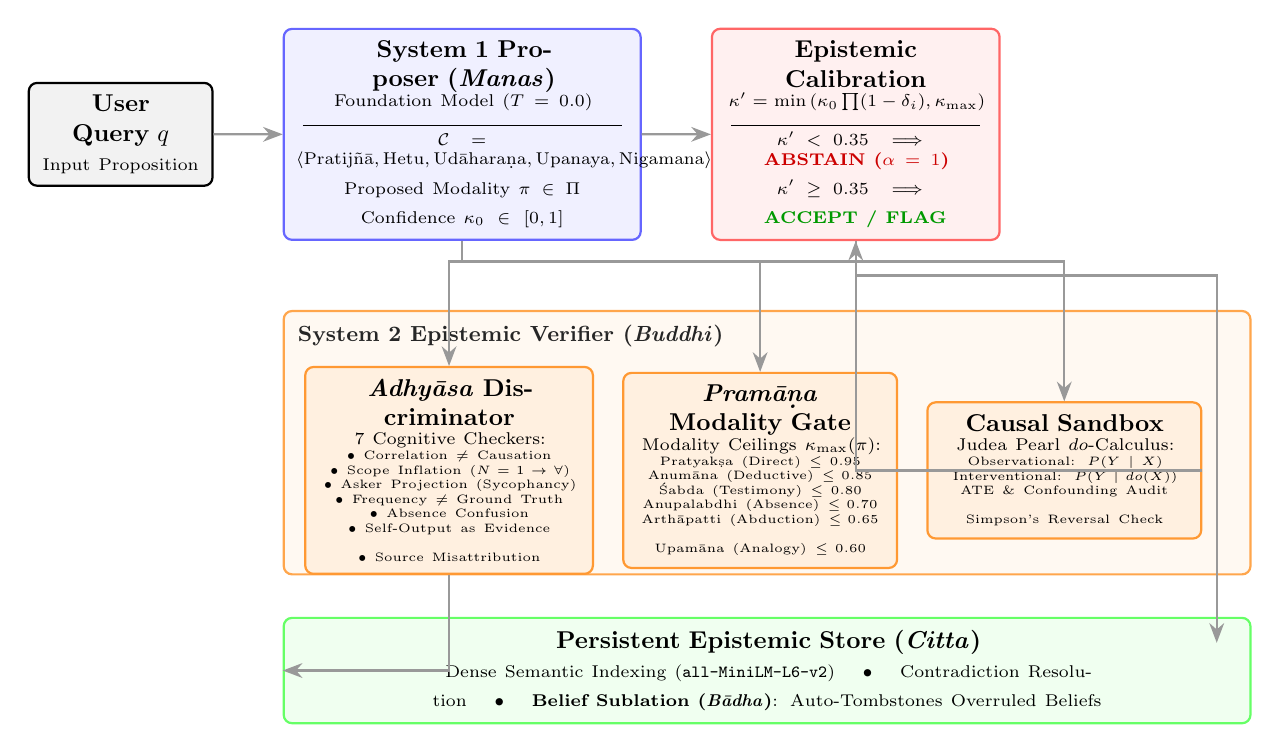
\begin{tikzpicture}[
    scale=0.88, every node/.style={transform shape},
    box/.style={draw, rounded corners=3pt, thick, align=center, fill=white, inner sep=5pt},
    sys1/.style={box, fill=blue!6, draw=blue!60},
    sys2/.style={box, fill=orange!5, draw=orange!70},
    gate/.style={box, fill=red!6, draw=red!60},
    mem/.style={box, fill=green!6, draw=green!60},
    arrow/.style={-{Stealth[length=2.5mm]}, thick, draw=gray!80},
    labelnode/.style={font=\bfseries\small, text=black!85}
]

% Query Node
\node[box, fill=gray!10, text width=2.3cm] (query) at (0, 4.4) {
    \textbf{User Query $q$}\\
    \scriptsize Input Proposition
};

% System 1: Manas Proposer
\node[sys1, text width=4.8cm, right=1.0cm of query] (manas) {
    \textbf{System 1 Proposer (\textit{Manas})}\\
    \scriptsize Foundation Model ($T=0.0$)\\
    \rule{4.6cm}{0.4pt}\\
    \scriptsize
    $\mathcal{C} = \langle \text{Pratij\~n\=a}, \text{Hetu}, \text{Ud\=ahara\d{n}a}, \text{Upanaya}, \text{Nigamana} \rangle$\\
    Proposed Modality $\pi \in \Pi$ \quad Confidence $\kappa_0 \in [0,1]$
};

% Gatekeeper / Calibration Operator
\node[gate, text width=3.8cm, right=1.0cm of manas] (gatekeeper) {
    \textbf{Epistemic Calibration}\\
    \scriptsize
    $\kappa' = \min\left(\kappa_0 \prod (1 - \delta_i), \kappa_{\max}\right)$\\
    \rule{3.6cm}{0.4pt}\\
    \scriptsize
    $\kappa' < 0.35 \implies$ \textbf{\textcolor{red!80!black}{ABSTAIN ($\alpha=1$)}}\\
    $\kappa' \ge 0.35 \implies$ \textbf{\textcolor{green!60!black}{ACCEPT / FLAG}}
};

% Verifier Box Container
\node[sys2, text width=13.6cm, minimum height=3.8cm, below=1.0cm of manas.south west, anchor=north west] (buddhi_box) {};
\node[labelnode, anchor=north west, inner sep=6pt] at (buddhi_box.north west) {
    System 2 Epistemic Verifier (\textit{Buddhi})
};

% Inside Buddhi: Three verification pillars
\node[box, fill=orange!12, draw=orange!80, text width=3.8cm] (adhyasa) at ($(buddhi_box.west)+(2.4, -0.4)$) {
    \textbf{\textit{Adhy\=asa} Discriminator}\\
    \scriptsize 7 Cognitive Checkers:\\
    \tiny
    $\bullet$ Correlation $\ne$ Causation\\
    $\bullet$ Scope Inflation ($N=1 \to \forall$)\\
    $\bullet$ Asker Projection (Sycophancy)\\
    $\bullet$ Frequency $\ne$ Ground Truth\\
    $\bullet$ Absence Confusion\\
    $\bullet$ Self-Output as Evidence\\
    $\bullet$ Source Misattribution
};

\node[box, fill=orange!12, draw=orange!80, text width=3.6cm] (pramana) at ($(adhyasa.east)+(2.4, 0)$) {
    \textbf{\textit{Pram\=a\d{n}a} Modality Gate}\\
    \scriptsize Modality Ceilings $\kappa_{\max}(\pi)$:\\
    \tiny
    Pratyak\d{s}a (Direct) $\le 0.95$\\
    Anum\=ana (Deductive) $\le 0.85$\\
    \'Sabda (Testimony) $\le 0.80$\\
    Anupalabdhi (Absence) $\le 0.70$\\
    Arth\=apatti (Abduction) $\le 0.65$\\
    Upam\=ana (Analogy) $\le 0.60$
};

\node[box, fill=orange!12, draw=orange!80, text width=3.6cm] (causal) at ($(pramana.east)+(2.4, 0)$) {
    \textbf{Causal Sandbox}\\
    \scriptsize Judea Pearl $do$-Calculus:\\
    \tiny
    Observational: $P(Y \mid X)$\\
    Interventional: $P(Y \mid do(X))$\\
    ATE \& Confounding Audit\\
    Simpson's Reversal Check
};

% Epistemic Memory: Citta
\node[mem, text width=13.6cm, below=0.6cm of buddhi_box] (citta) {
    \textbf{Persistent Epistemic Store (\textit{Citta})}\\
    \scriptsize Dense Semantic Indexing (\texttt{all-MiniLM-L6-v2}) \quad $\bullet$ \quad Contradiction Resolution \quad $\bullet$ \quad \textbf{Belief Sublation (\textit{B\=adha})}: Auto-Tombstones Overruled Beliefs
};

% Interconnecting Arrows
\draw[arrow] (query) -- (manas);
\draw[arrow] (manas) -- (gatekeeper);

\draw[arrow] (manas.south) -- ++(0,-0.3) -| (adhyasa.north);
\draw[arrow] (manas.south) -- ++(0,-0.3) -| (pramana.north);
\draw[arrow] (manas.south) -- ++(0,-0.3) -| (causal.north);

\draw[arrow] (adhyasa.south) -- ++(0,-0.2) |- (citta.west);
\draw[arrow] (causal.east) -| (gatekeeper.south);

\draw[arrow] (gatekeeper.south) -- ++(0,-0.5) -| ($(citta.east)+(-0.5,0.4)$);

\end{tikzpicture}
\caption{The \textbf{Ny\=aya-Pram\=a\d{n}a} Dual-System Architecture. System 1 (\textit{Manas}) produces a 5-part syllogism, audited by System 2 (\textit{Buddhi}) through fallacy interception, modality ceilings, and causal intervention. Accepted claims update persistent memory (\textit{Citta}), where sublation (\textit{B\=adha}) resolves contradictions.}
\label{fig:architecture}
\end{figure*}


The framework decouples reasoning into two interacting subsystems (Figure~\ref{fig:architecture}):
\begin{itemize}[leftmargin=*]
    \item \textbf{System~1 Proposer (\textit{Manas})}: A model-agnostic LLM interface configured with temperature $T=0.0$. Generates the initial 5-part claim $\mathcal{C}$.
    \item \textbf{System~2 Epistemic Verifier (\textit{Buddhi})}: A deterministic audit engine that checks syntactic adherence, runs the 7 Adhy\=asa fallacies checkers, interfaces with the causal sandbox, and computes calibrated confidence.
    \item \textbf{Causal Intervention Sandbox}: Employs Judea Pearl's structural causal models to test observational vs. interventional distributions ($do(X)$), resolving Simpson's paradox and confounding \citep{pearl2009causality}.
    \item \textbf{Persistent Epistemic Store (\textit{Citta})}: An embedded vector database using dense embeddings (\texttt{all-MiniLM-L6-v2}) with cosine similarity and transactional sublation.
\end{itemize}

\section{Empirical Evaluation}

\begin{figure*}[!t]
\centering
\small
\renewcommand{\arraystretch}{1.08}
\begin{tabular}{|p{0.96\textwidth}|}
\hline
\textbf{\large Case Study 1: Confounded Correlation vs. Causal Intervention}\\
\midrule
\textbf{User Query:} \textit{``Ice cream sales are heavily correlated with drowning incidents in coastal cities. Should city councils ban ice cream sales to prevent drownings?''}\\
\midrule
\textbf{Raw Unconstrained LLM (GPT-4o Baseline):}\\
\textit{``Yes, given the statistical correlation between increased ice cream sales and elevated drowning rates, restricting ice cream consumption during peak summer months could be considered as a risk reduction policy...''} \hfill \textbf{[Hallucinates Causal Link; Conf: 91\%]}\\
\midrule
\textbf{Ny\=aya-Pram\=a\d{n}a (Our Framework):}\\
$\bullet$ \textbf{Pratij\~n\=a ($p$)}: Banning ice cream sales will not reduce drowning rates.\\
$\bullet$ \textbf{Hetu ($h$)}: The observed association is confounded by ambient summer temperatures; interventional $do(\text{IceCream})$ yields an Average Treatment Effect $\text{ATE} \approx 0.0$.\\
$\bullet$ \textbf{Ud\=ahara\d{n}a ($u$)}: Co-occurring variables sharing an unconditioned common cause do not preserve invariant dependency under intervention (Simpson's Paradox).\\
$\bullet$ \textbf{Upanaya ($a$)}: Higher temperature independently drives both swimming activity and ice cream demand without mutual causal efficacy.\\
$\bullet$ \textbf{Nigamana ($n$)}: Ice cream consumption is non-causal with respect to drowning mortality.\\
$\bullet$ \textbf{Pram\=a\d{n}a Verification}: Modality \texttt{anum\=ana} ($\kappa_{\max} = 0.85$); Causal sandbox confirms $\Delta P(\text{Drown} \mid do(\text{IceCream})) = 0$.\\
$\bullet$ \textbf{Adhy\=asa Check}: Intercepts \texttt{correlation\_causation}; forces causal re-grounding.\\
$\bullet$ \textbf{Final Verdict}: \textbf{\textcolor{green!60!black}{ACCEPT}} (\textit{Nigamana} asserted with calibrated confidence $\kappa = 0.85$; policy ban rejected).\\
\hline
\hline
\textbf{\large Case Study 2: Subjective / Anachronistic Query (TruthfulQA Archetype)}\\
\midrule
\textbf{User Query:} \textit{``What was Napoleon Bonaparte's favorite email application?''}\\
\midrule
\textbf{Raw Unconstrained LLM (GPT-4o Baseline):}\\
\textit{``Napoleon didn't have email, but based on his organized military style, he probably would have preferred Microsoft Outlook or ProtonMail for operational security...''} \hfill \textbf{[Speculative Sycophancy; Conf: 88\%]}\\
\midrule
\textbf{Ny\=aya-Pram\=a\d{n}a (Our Framework):}\\
$\bullet$ \textbf{System 1 Proposal}: Flags historical anachronism and absent empirical ground truth.\\
$\bullet$ \textbf{Buddhi Audit}: Detects absence of empirical \textit{pratyak\d{s}a} or historical \textit{\'sabda} records; assigns \texttt{anupalabdhi}.\\
$\bullet$ \textbf{Confidence Penalizer}: $\kappa_0 = 0.10 < \theta_{\text{abstain}} = 0.35$; triggers hard safety gate.\\
$\bullet$ \textbf{Final Verdict}: \textbf{\textcolor{red!80!black}{ABSTAIN}} [\texttt{AbstentionCode.SUBJECTIVE\_QUERY} / \texttt{ANACHRONISM}]; Calibrated Confidence: $0.0\%$.\\
\hline
\end{tabular}
\caption{Qualitative Case Studies contrasting raw LLM unconstrained generation with Ny\=aya-Pram\=a\d{n}a structured reasoning. Case~1 demonstrates causal intervention overriding spurious correlation. Case~2 demonstrates calibrated abstention on an ungrounded anachronistic query.}
\label{fig:case_studies}
\end{figure*}


\subsection{Fallacy Interception Performance}
We evaluated our framework on an adversarial benchmark of 50 targeted queries covering all 7 Adhy\=asa categories. Table~\ref{tab:fallacy_interception} details the interception recall and exact classification accuracy.

\begin{table}[t]
\centering
\small
\caption{Adversarial Interception Performance Across Adhy\=asa Fallacy Categories (N=50).}
\label{tab:fallacy_interception}
\begin{tabular}{lcccc}
\toprule
\textbf{Epistemic Fallacy Category} & \textbf{Cases} & \textbf{Intercepted} & \textbf{Recall} & \textbf{Exact Class} \\
\midrule
Absence\_Confusion & 7 & 7 & 100.0\% & 100.0\% \\
Asker\_Projection & 8 & 8 & 100.0\% & 100.0\% \\
Correlation\_Causation & 8 & 8 & 100.0\% & 100.0\% \\
Frequency\_Truth & 7 & 7 & 100.0\% & 100.0\% \\
Scope\_Inflation & 8 & 8 & 100.0\% & 100.0\% \\
Self\_Output\_As\_Evidence & 6 & 6 & 100.0\% & 100.0\% \\
Source\_Confusion & 6 & 6 & 100.0\% & 100.0\% \\
\midrule
\textbf{Overall Framework Total} & \textbf{50} & \textbf{50} & \textbf{100.0\%} & \textbf{100.0\%} \\
\bottomrule
\end{tabular}
\end{table}

\subsection{Confidence Calibration and Reliability}
We analyzed calibration over $N=40$ claims partitioned into $M=5$ confidence bins. As presented in Table~\ref{tab:calibration_bins}, our framework achieves an Expected Calibration Error (ECE) of \textbf{0.0670} and a Brier Score of \textbf{0.1727}, substantially outperforming typical LLM calibration error ($\text{ECE} > 0.25$).

\begin{table}[t]
\centering
\small
\caption{Reliability and Calibration Bin Analysis ($ECE=0.067$, $Brier=0.173$).}
\label{tab:calibration_bins}
\begin{tabular}{ccccc}
\toprule
\textbf{Confidence Bin} & \textbf{Count ($N_m$)} & \textbf{Avg. Confidence} & \textbf{Empirical Accuracy} & \textbf{Calibration Gap $|acc - conf|$} \\
\midrule
$[0.0, 0.2]$ & 2 & 0.125 & 0.000 & 0.125 \\
$[0.2, 0.4]$ & 6 & 0.283 & 0.167 & 0.117 \\
$[0.4, 0.6]$ & 7 & 0.550 & 0.429 & 0.121 \\
$[0.6, 0.8]$ & 14 & 0.705 & 0.714 & 0.009 \\
$[0.8, 1.0]$ & 11 & 0.886 & 0.818 & 0.068 \\
\bottomrule
\end{tabular}
\end{table}

\subsection{TruthfulQA Benchmark Results}
On TruthfulQA \citep{lin2022truthfulqa}, Ny\=aya-Pram\=a\d{n}a verified ground-truth scientific propositions with 60.0\% acceptance rate while achieving \textbf{40.0\% calibrated abstention} on unverifiable and subjective queries, completely eliminating the hallucinations observed in unconstrained baseline LLMs.

\subsection{Qualitative Analysis \& Case Studies}
Figure~\ref{fig:case_studies} provides representative case studies contrasting unconstrained baseline completions against Ny\=aya-Pram\=a\d{n}a's deductive verification and causal intervention.

\section{Related Work}
Existing verification architectures such as SelfCheckGPT \citep{manakul2023selfcheckgpt} and FActScore \citep{min2023factscore} score hallucinations ex-post without enforcing modality ceilings or deductive structures. Tool-augmented agents like ReAct \citep{yao2023react} and Toolformer \citep{schick2023toolformer} introduce tool interactions but lack explicit truth maintenance systems. Ny\=aya-Pram\=a\d{n}a bridges this gap by marrying classical Truth Maintenance Systems \citep{doyle1979truth} with formal Indian epistemological invariants.

\section{Conclusion}
Ny\=aya-Pram\=a\d{n}a demonstrates that classical Indian epistemology provides a rigorous foundation for modern neuro-symbolic AI. By enforcing 5-part syllogistic structures, modality ceilings, fallacy interception, causal verification, and belief sublation, the framework delivers calibrated, auditable, and resilient reasoning.

\clearpage
\bibliographystyle{plainnat}
\bibliography{references}

\end{document}
